\documentclass[10pt]{article}
\usepackage{url}
\usepackage{xcolor}
\usepackage{rotating}
\usepackage{mdframed}
\usepackage{pdfpages}
\usepackage[papersize={12.865in,9.25in}, hmargin={.125in, .125in}, vmargin={1.25in,0in}]{geometry}

\newcommand{\hsc}[1]{{\footnotesize\MakeUppercase{#1}}}

 \definecolor{bg}{HTML}{F1E9D2}
 \pagecolor{bg}
% \pagecolor{black!8}
 \definecolor{nc}{HTML}{0C568C}

%parchment (greenish) F1F1D4 
 %parchment (better) F1E9D2 
%army green 95AB8A
%light blue CEE0F3
% beige FAFAF4
% dark blue 1E5F8F
\usepackage{tikz}
\usepackage{tkz-euclide}
\usetkzobj{all}
%\usetikzlibrary{calc}
\usepackage{pgfplots}
%\usetikzlibrary{shapes,calc,arrows,through,intersections,decorations.pathreplacing}
%\usepackage[T1]{fontenc}




\begin{document}

\pagestyle{empty}
\parbox{.4in}{
~
}
\parbox{4.5in}{
\pagestyle{empty}


\vskip -6em
~
\hspace{-4em}{\color{nc}Mathematics}

\vskip 3em

\noindent \parbox{3.2in}{
Motivated by questions in cosmology, {\em Geometry with an Introduction to Cosmic Topology} follows the Erlangen program to develop hyperbolic, elliptic, and Euclidean geometry - three possibilities for the global geometry of the universe.  
}
\parbox{.2in}{~}
\parbox{.8in}{
\begin{center}
\begin{tikzpicture}[scale=1, overlay]
	\tikzset{
		arrowMe/.style={postaction=decorate,
			decoration={markings, mark=at position .6 with {\arrow{#1}}
			} }}
	%\fill[color=brown!40](-3,-4) rectangle (3,4);
	%\fill[color=white](-1.1,-1.1) rectangle (1.1,1.1);
	%\draw[color=black] (-1.1,-1.1) rectangle (1.1,1.1);
	\clip (0,0) circle (1cm);
	\coordinate (o) at (0,0);
	\coordinate (a) at (1,0);
	\def\r{.8409};%this makes corner angles pi/4
	\fill[color=black!8] (o) circle (1cm);
	\tkzDrawCircle[dashed,color=blue](o,a)
	\foreach \x in {0,1,...,7} \tkzDefPoint(\x*45:\r){\x};
	\fill[color=yellow!30] 
	(0) to [bend left=44] (1) 
	to [bend left=44] (2) 
	to [bend left=44] (3) 
	to [bend left=44] (4) 
	to [bend left=44] (5) 
	to [bend left=44] (6) 
	to [bend left=44] (7) 
	to [bend left=44] (0) ;
	%%%The eight hyperbolic segments
	\tkzDefPointBy[inversion = center o through a](1)
	\tkzGetPoint{1s}
	\tkzCircumCenter(0,1,1s)\tkzGetPoint{c01}
	\tkzDrawArc[thick, color=orange](c01,1)(0)
	\tkzDefPointBy[inversion = center o through a](2)
	\tkzGetPoint{2s}
	\tkzCircumCenter(1,2,2s)\tkzGetPoint{c12}
	\tkzDrawArc[thick, color=blue](c12,2)(1)
	\tkzDefPointBy[inversion = center o through a](3)
	\tkzGetPoint{3s}
	\tkzCircumCenter(2,3,3s)\tkzGetPoint{c23}
	\tkzDrawArc[thick, color=red](c23,3)(2)
	\tkzDefPointBy[inversion = center o through a](4)
	\tkzGetPoint{4s}
	\tkzCircumCenter(3,4,4s)\tkzGetPoint{c34}
	\tkzDrawArc[thick, color=green](c34,4)(3)
	\tkzDefPointBy[inversion = center o through a](5)
	\tkzGetPoint{5s}
	\tkzCircumCenter(4,5,5s)\tkzGetPoint{c45}
	\tkzDrawArc[thick, color=red](c45,5)(4)
	\tkzDefPointBy[inversion = center o through a](6)
	\tkzGetPoint{6s}
	\tkzCircumCenter(5,6,6s)\tkzGetPoint{c56}
	\tkzDrawArc[thick, color=green](c56,6)(5)
	\tkzDefPointBy[inversion = center o through a](7)
	\tkzGetPoint{7s}
	\tkzCircumCenter(6,7,7s)\tkzGetPoint{c67}
	\tkzDrawArc[thick, color=orange](c67,7)(6)
	\tkzDefPointBy[inversion = center o through a](0)
	\tkzGetPoint{0s}
	\tkzCircumCenter(7,0,0s)\tkzGetPoint{c70}
	\tkzDrawArc[thick,color=blue](c70,0)(7)
	%%%%%Two points A and B  default (135:.6) and (275:.6)
	\def\theta{135};\def\r{.6};\def\alpha{260};\def\s{.4};
	\tkzDefPoint(\theta:\r){A}
	\tkzDefPoint(\alpha:\s){B}
	\tkzDefPointBy[inversion = center o through a](A)\tkzGetPoint{A*}
	\tkzDefPointBy[inversion = center o through a](B)\tkzGetPoint{B*}
	%%%%%Some paths from A to B
	%%Inside octagon
	\tkzCircumCenter(A,B,B*)\tkzGetPoint{center}
	\tkzDrawArc[thick](center,B)(A)
	%%Reflecting A and B across line L1 through origin at angle pi/8 to pos real axis
	\tkzDefPoint(45-\theta:\r){A1}
	\tkzDefPoint(45-\alpha:\s){B1}
	%%Reflecting A and B across line L2 through origin at angle 7pi/8 to pos real axis
	\tkzDefPoint(-45-\theta:\r){A2}
	\tkzDefPoint(-45-\alpha:\s){B2}
	%%T_d: transforming the octagon across first d edge: reflection by L1, inversion about circle containing this d edge 
	\tkzDefPointBy[inversion = center c56 through 5](A1)\tkzGetPoint{Ad*}
	\tkzDefPointBy[inversion = center c34 through 3](B1)\tkzGetPoint{Bd*}
	\tkzCircumCenter(A,A*,Bd*)\tkzGetPoint{centerd1}
	\tkzInterCC(c34,3)(centerd1,A)\tkzGetPoints{borderd1}{borderd2}
	\tkzCircumCenter(B,B*,Ad*)\tkzGetPoint{centerd2}
	\tkzInterCC(c56,5)(centerd2,B)\tkzGetPoints{borderd3}{borderd4}
	\tkzDrawArc[thick,color=green](centerd1,borderd2)(A)
	\tkzDrawArc[thick,color=green](centerd2,B)(borderd3)
	
	%%T_b: transforming the octagon across first b edge: reflection by L1, inversion about circle containing this b edge  
	\tkzDefPointBy[inversion = center c70 through 7](A1)\tkzGetPoint{Ab*}
	\tkzDefPointBy[inversion = center c12 through 1](B1)\tkzGetPoint{Bb*}
	\tkzCircumCenter(A,A*,Bb*)\tkzGetPoint{centerb1}
	\tkzInterCC(c12,1)(centerb1,A)\tkzGetPoints{borderb1}{borderb2}
	\tkzCircumCenter(B,B*,Ab*)\tkzGetPoint{centerb2}
	\tkzInterCC(c70,7)(centerb2,B)\tkzGetPoints{borderb3}{borderb4}
	\tkzDrawArc[thick,color=blue](centerb1,A)(borderb1)
	\tkzDrawArc[thick,color=blue](centerb2,borderb4)(B)
	
	
	%%T_c: transforming the octagon across first c edge: reflection by L2, inversion about circle containing this c edge 
	\tkzDefPointBy[inversion = center c45 through 5](A2)\tkzGetPoint{Ac*}
	\tkzDefPointBy[inversion = center c23 through 3](B2)\tkzGetPoint{Bc*}
	\tkzCircumCenter(A,A*,Bc*)\tkzGetPoint{centerc1}
	\tkzInterCC(c23,3)(centerc1,A)\tkzGetPoints{borderc1}{borderc2}
	\tkzCircumCenter(B,B*,Ac*)\tkzGetPoint{centerc2}
	\tkzInterCC(c45,5)(centerc2,B)\tkzGetPoints{borderc3}{borderc4}
	\tkzDrawArc[thick,color=red](centerc1,A)(borderc1)
	\tkzDrawArc[thick,color=red](centerc2,B)(borderc3)
	
	%%T_a: transforming the octagon across first a edge: reflection by L2, inversion about circle containing this a edge 
	\tkzDefPointBy[inversion = center c67 through 6](A2)\tkzGetPoint{Aa*}
	\tkzDefPointBy[inversion = center c01 through 1](B2)\tkzGetPoint{Ba*}
	\tkzCircumCenter(A,A*,Ba*)\tkzGetPoint{centera1}
	\tkzInterCC(c01,1)(centera1,A)\tkzGetPoints{bordera1}{bordera2}
	\tkzCircumCenter(B,B*,Aa*)\tkzGetPoint{centera2}
	\tkzInterCC(c67,6)(centera2,B)\tkzGetPoints{bordera3}{bordera4}
	\tkzDrawArc[thick,color=orange](centera1,A)(bordera1)
	\tkzDrawArc[thick,color=orange](centera2,bordera4)(B)
	
	\tkzDrawPoints[size=1,fill=red](0,1,2,3,4,5,6,7)
	\tkzDrawPoints[size=2,fill=blue](A,B)
	
	\foreach \t in {22.5,67.5,202.5,247.5} {\draw[arrowMe=stealth] (\t:.645)--(\t-.1:.645);}
	\foreach \t in {112.5,157.5,292.5,337.5} {\draw[arrowMe=stealth] (\t:.645)--(\t+.1:.645);}
	%\draw (22.5:.7) node{\Large\(a\)};
	%\draw (67.5:.7) node{\Large \(b\)};
	%\draw (112.5:.7) node{\Large\(c\)};
	%\draw (157.5:.7) node{\Large\(d\)};
	%\draw (202.5:.7) node{\Large\(c\)};
	%\draw (247.5:.72) node{\Large\(d\)};
	%\draw (292.5:.7) node{\Large\(a\)};
	%\draw (337.5:.7) node{\Large\(b\)};
	\end{tikzpicture}
\end{center}
}

\vskip1em
\noindent The text uses M\"obius transformations in the extended complex plane to define and investigate these three candidate geometries, thereby providing a natural setting in which to express results common to them all, as well as results that encapsulate key differences.  With these geometries in hand, the text then explores the interplay between the shape of a space and the type of geometry it admits.


\vskip2em
\noindent  The text has the following additional features:
\begin{itemize}
\item Geometric constructions play a central role in the development of the content, and Geometer's Sketchpad\textsuperscript{\textregistered} files for manipulating figures in non-Euclidean geometry are available at the text website.
\item It is written to be suitable for a one semester course in geometry or as a guide to independent study, with over 200 exercises and several essays on topics such as the history of geometry, parallax and curvature, and research aimed at determining the shape of the universe.
\item It is an open-content text, with low cost print editions and free electronic editions.
\end{itemize}

\vskip 2em
\noindent The most current version of the text can always be read online at 

\begin{center}
\url{http://mphitchman.com/}
\end{center}
}
\parbox{1in}{
~
}
\parbox{.615in}{

\begin{tikzpicture}
  \draw (0,8.5) node[rotate=-90] (author) {\Large \color{nc}\scshape Hitchman~~~~ \color{black}\scshape Geometry {\normalsize with an Introduction to} {\large Cosmic Topology}};
 \end{tikzpicture} 

\vskip1in
%\vfill
\hskip.7em
\begin{tikzpicture}[scale=.5, overlay]
	\tikzset{
		arrowMe/.style={postaction=decorate,
			decoration={markings, mark=at position .6 with {\arrow{#1}}
			} }}
	%\fill[color=brown!40](-3,-4) rectangle (3,4);
	%\fill[color=white](-1.1,-1.1) rectangle (1.1,1.1);
	%\draw[color=black] (-1.1,-1.1) rectangle (1.1,1.1);
	\clip (0,0) circle (1cm);
	\coordinate (o) at (0,0);
	\coordinate (a) at (1,0);
	\def\r{.8409};%this makes corner angles pi/4
	\fill[color=black!8] (o) circle (1cm);
	\tkzDrawCircle[dashed,color=blue](o,a)
	\foreach \x in {0,1,...,7} \tkzDefPoint(\x*45:\r){\x};
	\fill[color=yellow!30] 
	(0) to [bend left=44] (1) 
	to [bend left=44] (2) 
	to [bend left=44] (3) 
	to [bend left=44] (4) 
	to [bend left=44] (5) 
	to [bend left=44] (6) 
	to [bend left=44] (7) 
	to [bend left=44] (0) ;
	%%%The eight hyperbolic segments
	\tkzDefPointBy[inversion = center o through a](1)
	\tkzGetPoint{1s}
	\tkzCircumCenter(0,1,1s)\tkzGetPoint{c01}
	\tkzDrawArc[thick, color=orange](c01,1)(0)
	\tkzDefPointBy[inversion = center o through a](2)
	\tkzGetPoint{2s}
	\tkzCircumCenter(1,2,2s)\tkzGetPoint{c12}
	\tkzDrawArc[thick, color=blue](c12,2)(1)
	\tkzDefPointBy[inversion = center o through a](3)
	\tkzGetPoint{3s}
	\tkzCircumCenter(2,3,3s)\tkzGetPoint{c23}
	\tkzDrawArc[thick, color=red](c23,3)(2)
	\tkzDefPointBy[inversion = center o through a](4)
	\tkzGetPoint{4s}
	\tkzCircumCenter(3,4,4s)\tkzGetPoint{c34}
	\tkzDrawArc[thick, color=green](c34,4)(3)
	\tkzDefPointBy[inversion = center o through a](5)
	\tkzGetPoint{5s}
	\tkzCircumCenter(4,5,5s)\tkzGetPoint{c45}
	\tkzDrawArc[thick, color=red](c45,5)(4)
	\tkzDefPointBy[inversion = center o through a](6)
	\tkzGetPoint{6s}
	\tkzCircumCenter(5,6,6s)\tkzGetPoint{c56}
	\tkzDrawArc[thick, color=green](c56,6)(5)
	\tkzDefPointBy[inversion = center o through a](7)
	\tkzGetPoint{7s}
	\tkzCircumCenter(6,7,7s)\tkzGetPoint{c67}
	\tkzDrawArc[thick, color=orange](c67,7)(6)
	\tkzDefPointBy[inversion = center o through a](0)
	\tkzGetPoint{0s}
	\tkzCircumCenter(7,0,0s)\tkzGetPoint{c70}
	\tkzDrawArc[thick,color=blue](c70,0)(7)
	%%%%%Two points A and B  default (135:.6) and (275:.6)
	\def\theta{135};\def\r{.6};\def\alpha{260};\def\s{.4};
	\tkzDefPoint(\theta:\r){A}
	\tkzDefPoint(\alpha:\s){B}
	\tkzDefPointBy[inversion = center o through a](A)\tkzGetPoint{A*}
	\tkzDefPointBy[inversion = center o through a](B)\tkzGetPoint{B*}
	%%%%%Some paths from A to B
	%%Inside octagon
	\tkzCircumCenter(A,B,B*)\tkzGetPoint{center}
	\tkzDrawArc[thick](center,B)(A)
	%%Reflecting A and B across line L1 through origin at angle pi/8 to pos real axis
	\tkzDefPoint(45-\theta:\r){A1}
	\tkzDefPoint(45-\alpha:\s){B1}
	%%Reflecting A and B across line L2 through origin at angle 7pi/8 to pos real axis
	\tkzDefPoint(-45-\theta:\r){A2}
	\tkzDefPoint(-45-\alpha:\s){B2}
	%%T_d: transforming the octagon across first d edge: reflection by L1, inversion about circle containing this d edge 
	\tkzDefPointBy[inversion = center c56 through 5](A1)\tkzGetPoint{Ad*}
	\tkzDefPointBy[inversion = center c34 through 3](B1)\tkzGetPoint{Bd*}
	\tkzCircumCenter(A,A*,Bd*)\tkzGetPoint{centerd1}
	\tkzInterCC(c34,3)(centerd1,A)\tkzGetPoints{borderd1}{borderd2}
	\tkzCircumCenter(B,B*,Ad*)\tkzGetPoint{centerd2}
	\tkzInterCC(c56,5)(centerd2,B)\tkzGetPoints{borderd3}{borderd4}
	\tkzDrawArc[thick,color=green](centerd1,borderd2)(A)
	\tkzDrawArc[thick,color=green](centerd2,B)(borderd3)
	
	%%T_b: transforming the octagon across first b edge: reflection by L1, inversion about circle containing this b edge  
	\tkzDefPointBy[inversion = center c70 through 7](A1)\tkzGetPoint{Ab*}
	\tkzDefPointBy[inversion = center c12 through 1](B1)\tkzGetPoint{Bb*}
	\tkzCircumCenter(A,A*,Bb*)\tkzGetPoint{centerb1}
	\tkzInterCC(c12,1)(centerb1,A)\tkzGetPoints{borderb1}{borderb2}
	\tkzCircumCenter(B,B*,Ab*)\tkzGetPoint{centerb2}
	\tkzInterCC(c70,7)(centerb2,B)\tkzGetPoints{borderb3}{borderb4}
	\tkzDrawArc[thick,color=blue](centerb1,A)(borderb1)
	\tkzDrawArc[thick,color=blue](centerb2,borderb4)(B)
	
	
	%%T_c: transforming the octagon across first c edge: reflection by L2, inversion about circle containing this c edge 
	\tkzDefPointBy[inversion = center c45 through 5](A2)\tkzGetPoint{Ac*}
	\tkzDefPointBy[inversion = center c23 through 3](B2)\tkzGetPoint{Bc*}
	\tkzCircumCenter(A,A*,Bc*)\tkzGetPoint{centerc1}
	\tkzInterCC(c23,3)(centerc1,A)\tkzGetPoints{borderc1}{borderc2}
	\tkzCircumCenter(B,B*,Ac*)\tkzGetPoint{centerc2}
	\tkzInterCC(c45,5)(centerc2,B)\tkzGetPoints{borderc3}{borderc4}
	\tkzDrawArc[thick,color=red](centerc1,A)(borderc1)
	\tkzDrawArc[thick,color=red](centerc2,B)(borderc3)
	
	%%T_a: transforming the octagon across first a edge: reflection by L2, inversion about circle containing this a edge 
	\tkzDefPointBy[inversion = center c67 through 6](A2)\tkzGetPoint{Aa*}
	\tkzDefPointBy[inversion = center c01 through 1](B2)\tkzGetPoint{Ba*}
	\tkzCircumCenter(A,A*,Ba*)\tkzGetPoint{centera1}
	\tkzInterCC(c01,1)(centera1,A)\tkzGetPoints{bordera1}{bordera2}
	\tkzCircumCenter(B,B*,Aa*)\tkzGetPoint{centera2}
	\tkzInterCC(c67,6)(centera2,B)\tkzGetPoints{bordera3}{bordera4}
	\tkzDrawArc[thick,color=orange](centera1,A)(bordera1)
	\tkzDrawArc[thick,color=orange](centera2,bordera4)(B)
	
	\tkzDrawPoints[size=1,fill=red](0,1,2,3,4,5,6,7)
	\tkzDrawPoints[size=2,fill=blue](A,B)
	
	%\foreach \t in {22.5,67.5,202.5,247.5} {\draw[arrowMe=stealth] (\t:.645)--(\t-.1:.645);}
	%\foreach \t in {112.5,157.5,292.5,337.5} {\draw[arrowMe=stealth] (\t:.645)--(\t+.1:.645);}
	\end{tikzpicture}
}
\parbox{.3in}{~}
\parbox{5in}{
~
\vskip3.7in
\begin{center}
%\vskip2.5in
	\begin{tikzpicture}[scale=3.5, overlay]
		\tikzset{
		arrowMe/.style={postaction=decorate,
			decoration={markings, mark=at position .5 with {\arrow[very thick]{#1}}
			} }}
	%\fill[color=brown!40](-3,-4) rectangle (3,4);
	%\fill[color=brown!20](-1.1,-1.1) rectangle (1.1,1.1);
	%\draw[very thick,color=black] (-1.1,-1.1) rectangle (1.1,1.1);
	\clip (0,0) circle (1cm);
	\coordinate (o) at (0,0);
	\coordinate (a) at (1,0);
	\def\r{.8409};%this makes corner angles pi/4
	\fill[color=black!8] (o) circle (1cm);
	\tkzDrawCircle[very thick, dashed,color=blue](o,a)
	\foreach \x in {0,1,...,7} \tkzDefPoint(\x*45:\r){\x};
	\fill[color=yellow!30] 
	(0) to [bend left=44] (1) 
	to [bend left=44] (2) 
	to [bend left=44] (3) 
	to [bend left=44] (4) 
	to [bend left=44] (5) 
	to [bend left=44] (6) 
	to [bend left=44] (7) 
	to [bend left=44] (0) ;
	%%%The eight hyperbolic segments
	\tkzDefPointBy[inversion = center o through a](1)
	\tkzGetPoint{1s}
	\tkzCircumCenter(0,1,1s)\tkzGetPoint{c01}
	\tkzDrawArc[thick, color=orange](c01,1)(0)
	\tkzDefPointBy[inversion = center o through a](2)
	\tkzGetPoint{2s}
	\tkzCircumCenter(1,2,2s)\tkzGetPoint{c12}
	\tkzDrawArc[thick, color=blue](c12,2)(1)
	\tkzDefPointBy[inversion = center o through a](3)
	\tkzGetPoint{3s}
	\tkzCircumCenter(2,3,3s)\tkzGetPoint{c23}
	\tkzDrawArc[thick, color=red](c23,3)(2)
	\tkzDefPointBy[inversion = center o through a](4)
	\tkzGetPoint{4s}
	\tkzCircumCenter(3,4,4s)\tkzGetPoint{c34}
	\tkzDrawArc[thick, color=green](c34,4)(3)
	\tkzDefPointBy[inversion = center o through a](5)
	\tkzGetPoint{5s}
	\tkzCircumCenter(4,5,5s)\tkzGetPoint{c45}
	\tkzDrawArc[thick, color=red](c45,5)(4)
	\tkzDefPointBy[inversion = center o through a](6)
	\tkzGetPoint{6s}
	\tkzCircumCenter(5,6,6s)\tkzGetPoint{c56}
	\tkzDrawArc[thick, color=green](c56,6)(5)
	\tkzDefPointBy[inversion = center o through a](7)
	\tkzGetPoint{7s}
	\tkzCircumCenter(6,7,7s)\tkzGetPoint{c67}
	\tkzDrawArc[thick, color=orange](c67,7)(6)
	\tkzDefPointBy[inversion = center o through a](0)
	\tkzGetPoint{0s}
	\tkzCircumCenter(7,0,0s)\tkzGetPoint{c70}
	\tkzDrawArc[thick,color=blue](c70,0)(7)
	%%%%%Two points A and B  default (135:.6) and (275:.6)
	\def\theta{135};\def\r{.6};\def\alpha{260};\def\s{.4};
	\tkzDefPoint(\theta:\r){A}
	\tkzDefPoint(\alpha:\s){B}
	\tkzDefPointBy[inversion = center o through a](A)\tkzGetPoint{A*}
	\tkzDefPointBy[inversion = center o through a](B)\tkzGetPoint{B*}
	%%%%%Some paths from A to B
	%%Inside octagon
	\tkzCircumCenter(A,B,B*)\tkzGetPoint{center}
	\tkzDrawArc[thick](center,B)(A)
	%%Reflecting A and B across line L1 through origin at angle pi/8 to pos real axis
	\tkzDefPoint(45-\theta:\r){A1}
	\tkzDefPoint(45-\alpha:\s){B1}
	%%Reflecting A and B across line L2 through origin at angle 7pi/8 to pos real axis
	\tkzDefPoint(-45-\theta:\r){A2}
	\tkzDefPoint(-45-\alpha:\s){B2}
	%%T_d: transforming the octagon across first d edge: reflection by L1, inversion about circle containing this d edge 
	\tkzDefPointBy[inversion = center c56 through 5](A1)\tkzGetPoint{Ad*}
	\tkzDefPointBy[inversion = center c34 through 3](B1)\tkzGetPoint{Bd*}
	\tkzCircumCenter(A,A*,Bd*)\tkzGetPoint{centerd1}
	\tkzInterCC(c34,3)(centerd1,A)\tkzGetPoints{borderd1}{borderd2}
	\tkzCircumCenter(B,B*,Ad*)\tkzGetPoint{centerd2}
	\tkzInterCC(c56,5)(centerd2,B)\tkzGetPoints{borderd3}{borderd4}
	\tkzDrawArc[thick,color=green](centerd1,borderd2)(A)
	\tkzDrawArc[thick,color=green](centerd2,B)(borderd3)
	
	%%T_b: transforming the octagon across first b edge: reflection by L1, inversion about circle containing this b edge  
	\tkzDefPointBy[inversion = center c70 through 7](A1)\tkzGetPoint{Ab*}
	\tkzDefPointBy[inversion = center c12 through 1](B1)\tkzGetPoint{Bb*}
	\tkzCircumCenter(A,A*,Bb*)\tkzGetPoint{centerb1}
	\tkzInterCC(c12,1)(centerb1,A)\tkzGetPoints{borderb1}{borderb2}
	\tkzCircumCenter(B,B*,Ab*)\tkzGetPoint{centerb2}
	\tkzInterCC(c70,7)(centerb2,B)\tkzGetPoints{borderb3}{borderb4}
	\tkzDrawArc[thick,color=blue](centerb1,A)(borderb1)
	\tkzDrawArc[thick,color=blue](centerb2,borderb4)(B)
	
	
	%%T_c: transforming the octagon across first c edge: reflection by L2, inversion about circle containing this c edge 
	\tkzDefPointBy[inversion = center c45 through 5](A2)\tkzGetPoint{Ac*}
	\tkzDefPointBy[inversion = center c23 through 3](B2)\tkzGetPoint{Bc*}
	\tkzCircumCenter(A,A*,Bc*)\tkzGetPoint{centerc1}
	\tkzInterCC(c23,3)(centerc1,A)\tkzGetPoints{borderc1}{borderc2}
	\tkzCircumCenter(B,B*,Ac*)\tkzGetPoint{centerc2}
	\tkzInterCC(c45,5)(centerc2,B)\tkzGetPoints{borderc3}{borderc4}
	\tkzDrawArc[thick,color=red](centerc1,A)(borderc1)
	\tkzDrawArc[thick,color=red](centerc2,B)(borderc3)
	
	%%T_a: transforming the octagon across first a edge: reflection by L2, inversion about circle containing this a edge 
	\tkzDefPointBy[inversion = center c67 through 6](A2)\tkzGetPoint{Aa*}
	\tkzDefPointBy[inversion = center c01 through 1](B2)\tkzGetPoint{Ba*}
	\tkzCircumCenter(A,A*,Ba*)\tkzGetPoint{centera1}
	\tkzInterCC(c01,1)(centera1,A)\tkzGetPoints{bordera1}{bordera2}
	\tkzCircumCenter(B,B*,Aa*)\tkzGetPoint{centera2}
	\tkzInterCC(c67,6)(centera2,B)\tkzGetPoints{bordera3}{bordera4}
	\tkzDrawArc[thick,color=orange](centera1,A)(bordera1)
	\tkzDrawArc[thick,color=orange](centera2,bordera4)(B)
	
	\tkzDrawPoints[size=3,fill=red](0,1,2,3,4,5,6,7)
	\tkzDrawPoints[size=5,fill=blue](A,B)
	
	\foreach \t in {22.5,67.5,202.5,247.5} {\draw[arrowMe=stealth] (\t:.645)--(\t-.1:.645);}
	\foreach \t in {112.5,157.5,292.5,337.5} {\draw[arrowMe=stealth] (\t:.645)--(\t+.1:.645);}
	%\draw (22.5:.7) node{\Large\(a\)};
	%\draw (67.5:.7) node{\Large \(b\)};
	%\draw (112.5:.7) node{\Large\(c\)};
	%\draw (157.5:.7) node{\Large\(d\)};
	%\draw (202.5:.7) node{\Large\(c\)};
	%\draw (247.5:.72) node{\Large\(d\)};
	%\draw (292.5:.7) node{\Large\(a\)};
	%\draw (337.5:.7) node{\Large\(b\)};
	\end{tikzpicture}
	
	\vskip-3.9in
	
	\resizebox{.9\linewidth}{!}{\color{nc}  \scshape Geometry}
	
	\vskip.3in
	
	\resizebox{.7\linewidth}{!}{\color{black!80} \scshape with an Introduction to}
	
	\vskip.2in
	\resizebox{.7\linewidth}{!}{\color{nc} \scshape Cosmic Topology}
	
	\vskip.5in
	\resizebox{.3\linewidth}{!}{\color{black!80}  \scshape 2018 Edition}

	\vskip3.5in


	\resizebox{.75\linewidth}{!}{\color{nc}\scshape Michael P. Hitchman}
	
	%%%% Sans Serif Workup
%	\vskip-3.6in
%	\sffamily
%	\resizebox{.85\linewidth}{!}{\color{nc}  G\hsc{eometry}}
%	
%	\vskip.3in
%	
%	\resizebox{.7\linewidth}{!}{\color{black!80} \hsc{with an} I\hsc{ntroduction to}}
%	
%	\vskip.2in
%	\resizebox{.7\linewidth}{!}{\color{black}  C\hsc{osmic} T\hsc{opology}}
%	
%	\vskip.2in
%	\resizebox{.3\linewidth}{!}{\color{black!80}   2018 E\hsc{dition}}
%
%	\vskip3.8in
%
%
%	\resizebox{.75\linewidth}{!}{\color{nc} M\hsc{ichael} P. H\hsc{itchman}}
\end{center}
}
\parbox{.75in}{~}

\thispagestyle{empty}
\clearpage
\end{document}